\section{\centerline{Introduction}}
\label{sec:introduction}

\vspace {15pt}
Electroencephalogram (EEG) is the recording of electrical signals from the scalp, representing the electrical activity of the brain. EEG is used for decades as a medical tool to diagnose brain diseases such as epilepsy, as well as a diagnostic test in psychiatry. EEG signals are also used in Brain Computer Interface (BCI) systems, most of which are based on motor imagery resulting in movement execution. Examples of BCI applications are the control of the operation of a wheelchair, or a robot arm, as well as in games as the user interface. In BCI systems, decisions are made based on consciously generated EEG signals by the user. BCI are closed loop systems, since the user observes the effect on the device to be controlled and in a way adjusts his brain activity accordingly. Through this process a user can become more effective in the control of a device through practice.  
 
EEG signals are subject to noise which in some cases has amplitude much greater than the amplitude of the desired EEG signal. For a successful BCI operation, this noise must be removed or avoided, since the noise can result in a false detection of the user’s intention. The ability of a BCI system to detect the user’s intent with a correct decision made depends also on other factors such as the number of electrodes used to record the EEG signals, the scalp positions they are placed, since different scalp positions are more suitable for detecting different brain activities, as well as on the EEG signal frequencies examined.
 
The purpose of this project is to investigate the capability of EEG signals in providing the necessary information for the detection of the user’s intention in BCI systems, when using a single electrode connected to the Fp1 position of the scalp. This investigation includes the recordings of EEG signals produced by willing persons, consciously performing a mental task such as trying to move an object on the screen of a computer, as well as the analysis of the power spectrum of the EEG signals in the alpha frequency band (8Hz to 12Hz) and the computation of the signal-to-noise ratio (SNR).   

\subsection{\bf{Noise in EEG signals:}}

The strength of EEG signals is very small, in the order of microvolts. EEG signals suffer from noise, which in some cases has amplitude much greater than the signal amplitude. This noise can be either due to the external noise generated by electrical devices, such as the 50Hz mains noise, or due to body muscular activity, known as the artefacts. Possible sources of artefacts, are activities from other parts of the body that generate electrical signals, such as the noise due to eye movement and eye blinking, heart activity and facial muscle movements  \citep{Yong2008}. Furthermore, EEG signals contain information on the conscious intent of the subject, as well as other signals due to brain activity not related to the specific intent of the subject. These other signals can also be treated as noise, since they affect the accuracy of decision making on the subject’s intent. This noise is usually called the background noise. In BCI conscious applications, in order to be able to analyse EEG signals correctly and obtain a successful decision, it is essential that noise is removed, or discard the recorded data for the duration during which the artefact is detected  \citep{Balbir2017,Repovs2010}. The option of discarding the EEG signal segments when noise is detected in not always possible. For example EEG background EEG is always present.  

In theory, the information from a noisy EEG signal can be correctly extracted, given that a minimum number of signal samples are used, or the signal is examine for a minimum time duration. This implies that as the SNR of the EEG signal decreases, the required number of samples or the signal duration must be increased. If the SNR becomes very low, then the number of required samples or the signal time duration becomes infinite. Therefore, there is a minimum limit of the SNR, beyond which the signal information cannot be correctly determined, called the SNR Wall \citep{Tandra2008a,Kustra2017,Tandra2008b}. A study on the SNR Wall in relation to the SNR of EEG signals has already been done at the University of Glasgow during the academic year 2017-2018 \citep{Porr2018}. This study included the development of the methodology and the mathematical equations needed to compute the SNR wall and the SNR for the recorded signals for various settings, such as eye blink, smile and reading aloud a text. In this work, the EEG and the electromyography (EMG) signals due to artefacts are considered as noise and the SNR calculations are done based on the energy of the artefact EEG/EMG signals. For the calculation of the SNR signal power is considered to be the conscious change in EEG power from paralyzed persons \citep{Whitham2007}.
    
\subsection{\bf{Project Aims and Objectives:}}
The aim of this project is to develop a methodology that enables the investigation of the capability of EEG signals in providing the necessary information for the detection of the user’s intention when using a single electrode connected to the Fp1 position of the scalp. More specifically, the objectives of this project are to:

\begin{enumerate}
	\item Produce a literature review on the main issues related to the work of the project. This review will concentrate on motor imagery BCI systems.
	\item	Setup and configure a BCI hardware consisting of an EEG signal amplifier and a 24-bit sigma-delta A/D converter board. This hardware is based on existing boards available by the University of Glasgow. 
	\item	Devise experimental settings and perform a number of experiments that will enable the recording of EEG signals from a number of persons who will consciously try to perform a brain function, such as trying to move an object on the screen of a computer, or attempting to increase their own 10Hz peak in their EEG spectrum. 
	\item	Devise the methodology and build the necessary software that will enable the analysis of the conscious EEG signals recorded.
	\item	Analyse the recorded EEG with respect to their SNR characteristics, in order to determine whether EEG signals in the alpha frequency zone, obtained from a single electrode connected to Fp1 position on the scalp can be safely used by BCI systems to determine the intent of a user. 
\end{enumerate}

\subsection{\bf{Project Methodology:}}
For the purpose of this project, the analysis of the EEG signals and the estimation of the intent of the person will be based on the time domain and the frequency spectrum of the EEG signals. Earlier research work has shown a relationship between the person’s intent and the frequency band of the EEG signals \citep{Wolpaw1991,Wolpaw2004}. Other parameters that could affect the analysis of the EEG signals, are the number of electrodes (sensors) used and the scalp position of the electrodes. This project examines the EEG signals in the alpha frequency band (8Hz to 12Hz) taken from an electrode connected to the Fp1 position. This emulates a typical EEG gadget for gaming control.

To investigate the EEG signals in the alpha wave frequency band taken from an electrode connected to the Fp1 position and the achieved SNR, experiments were done with a person referred to as the subject. The experiments were conducted with a data acquisition system consisting of the EEG electrodes, a custom made signal amplifier with a voltage gain of 50, and the “USB DUX SIGMA” 24-bit analogue-to-digital converter board (Porr, B linux-usb-daq.co.uk). EEG recordings were made using the open source software “Comedirecord” (Porr B. , ComediRecord). This software enables the acquisition of signals, signal filtering, display of time domain signal, display of the frequency spectrum and the recording of the raw signal.
 
 During the experiment’s procedure, the subject was performing a mental task, such as trying to move an object on screen of a computer, while at the same time observing the 10Hz peak of the real time spectrum of the generated EEG signal on the screen of the computer. The EEG signals generated by the subject were recorded on a computer. This enables a closed loop control of the BCI system. The subjects were looking at their own Fourier spectrum and trying to consciously maximize the alpha band frequency peak, thus achieving maximum SNR.

The recorded EEG signals were filtered to remove any external noise, such as the 50Hz mains noise. To isolate the alpha band frequencies, the EEG recordings were also filtered by a bandpass filter. The SNR wall was calculated for each subject using as noise signal the first part of the recording of each experiment for the specific subject. This part of the signal corresponds to the time period that the subject is relaxed. This calculation was achieved using the maximum and the minimum variances between the recordings of the different experiments. The calculation of the SNR was based on the information signal which is the EEG signal during the instances that a person is consciously performing a mental operation, while the noise was the background EEG noise signal obtained when the person was relaxed, doing nothing. For each experiment, the SNR was compared to the SNR wall in order to specify whether a detection can be made or not. The power of the EEG signal related to the intent of the subject was varying during the time of the effort of the subject. For this reason, the SNR was calculated for signal segments corresponding to one-second time periods, with a 500ms time difference between adjacent signal segments. The proposed methodology can help in identifying the instance during which the SNR is maximum and therefore, use this EEG signal segment for the decision on the subject’s intent.

The subjects were instructed to avoid any intentional movements that could create artefacts. In the case that artefacts ware identified in the EEG recordings, the signal segment corresponding to the duration of the artefact was ignored.
   
\subsection{\bf{Background Theory:}}
Electroencephalography (EEG) refers to the recordings of the electrical activity of the brain. The origins of EEG dates back in 1875 when Richard Caton observed EEG signal activity in exposed brains of animals. The first EEG recordings in humans were reported by Hans Berger in 1924. EEG has evolved since then and is currently used in clinical applications to detect coma and brain death, to locate brain areas damaged after head injury or stroke, to control anesthesia depth, to investigate epilepsy and seizure, to investigate sleep disorders and many other applications. EEG is also the means of providing information on the user’s intent in Brain Computer Interfaces (BCI) used to control the operation of actuators in devices such as wheelchairs and human prosthetic limbs, as well as in gaming. 

\subsubsection{\bf{EEG Signals:}}
EEG signals are electrical signals representing brain activity. When EEG signals are obtained through specialized electrodes attached on the scalp, the process used is referred to as non-invasive. Due to the fact that in non-invasive EEG the electrical signals are taken from the scalp, EEG signals are weak, in the order of microvolts (µV). To improve the quality of the recorded EEG signals the electrodes are placed on the scalp using a conductive gel. Furthermore, the scalp area is prepared with a light abrasion to remove dead skin cells and thus reduce the scalp impedance. In many systems the electrodes are embedded on caps or nets. 
Information deduced from EEG signals depends on the scalp position where the electrodes are attached. This is due to the fact that different parts of the brain are related to different brain activities. Therefore, mapping schemes are used to identify the scalp positions where electrodes can be attached. A common mapping scheme widely used is the “International 10-20” scheme \citep{Towle1993}, shown in Figure \ref{I20map}. 


\begin{figure}
	\centering
%	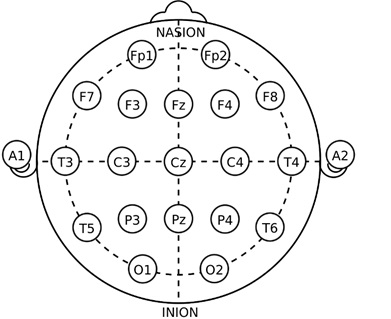
\includegraphics[width=\linewidth]{Figures/Brain_I20.jpg} % Figure image
	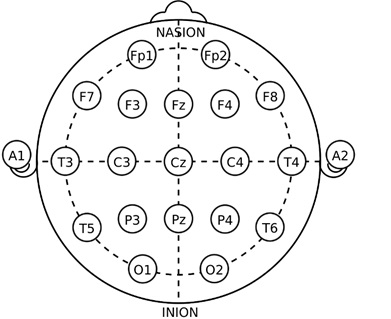
\includegraphics[width=8cm]{Figures/Brain_I20.jpg} % Figure image
	\caption{The International 10-20 mapping} % Figure caption
	\label{I20map} % Label for referencing with \ref{bear}
\end{figure}

% \begin{enumerate}[label=\alph*.] \item Blablah 1 \item Blablah 2 \item Blablah 3 ...


Another factor that relates to the information conveyed by EEG signals is the EEG rhythmic activity, identified in different frequency bands \citep{Fink2014}. These frequency bands are the following:

\begin{enumerate} [label=\alph*)]
	\item Delta (<4Hz) 
	\item Theta (4Hz to 7Hz)
	\item Alpha (8Hz to 12Hz) 
	\item Beta (12Hz to 30Hz)
	\item Gamma (>31Hz)
	\item Mu (8Hz to 12Hz)  
\end{enumerate} 

The Alpha frequency band is also referred to occupy the frequency range from 8Hz to 15Hz in bibliography. The Mu frequency band overlaps with the alpha frequency band and refers to the EEG signals taken from the motor cortex (C3, Cz, and C4 electrode positions).  

Decoding brain activity is a function of both the frequency band examined and the electrode positions used to record the EEG signals. When performing a motor task, or imagine of a motor task the energy from the mu (alpha) and the beta rhythms will rise or fall. Event related synchronization (ERS) refers to the case when the energy rises, while event related desynchronization (ERD) refers to the case when the energy falls. ERD in the mu band is observed during the performance of a motor task. This is known as the mu suppression. ERD occurs also by observing a motor action carried out by another person. A study of the mu suppression on different areas of the alpha band frequency (8Hz to 10Hz and 10Hz to 12Hz) prior and during hand/foot movements showed a higher mu suppression in the lower frequencies \citep{Pfurtscheller2000}.  A study in \citep{Khulman1978} showed that manual execution resulted in a maximum ERD at the frequency of 10.1Hz. The effect in ERD when performing and observing manual movements with respect to frequency ranges in the alpha frequency band and the spatial domains is examined in \citep{Frenkel2013}. The effect of ERD when performing or observing hand movements is shown in Figure \ref{Scalp}. 


\begin{figure}
	\centering
	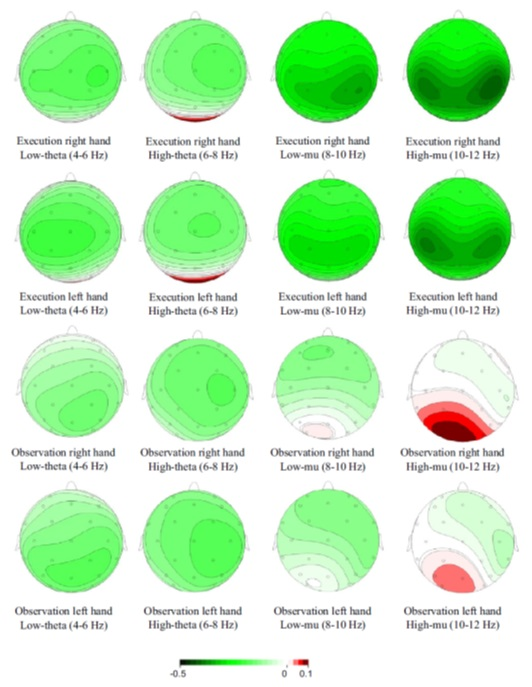
\includegraphics[width=\linewidth]{Figures/ScalpSignals.jpg} % Figure image
%	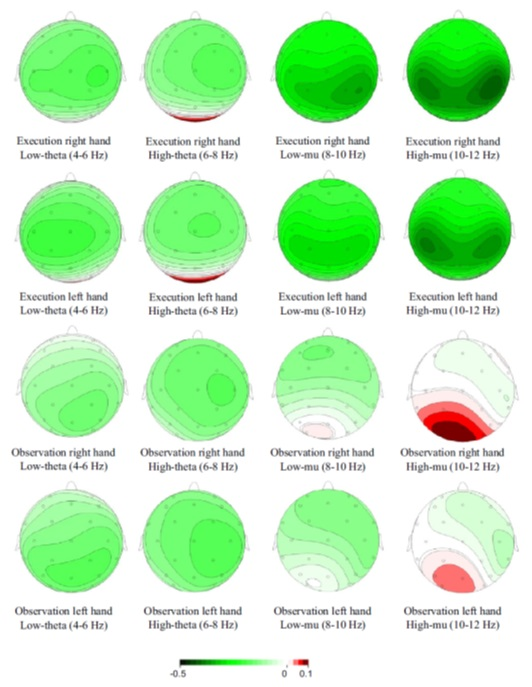
\includegraphics[width=14cm]{Figures/ScalpSignals.jpg} % Figure image
	\caption{The scalp distribution of suppression in the different execution and observation conditions. (Figure taken from \citep{Frenkel2013}.} 
	\label{Scalp} % Label for referencing with \ref{bear}
\end{figure}


\subsubsection{\bf{Noise in EEG Signals:}}
EEG signals are contaminated by noise. EEG noise is considered to be any EEG electrical signal recorded that is the signal amplifier is place not produced by brain activity. This noise can be externally produced by external sources such as electrical or electronic devices, or produced by the movements of the electrode assembly. Another source of noise in EEG is the noise due to the operation and activities of the human body, such as smiling or eye movement, referred to as the artefacts. In the study and decoding of EEG recordings, signals due to brain activity not related to the activity examined are often assumed and treated as noise.    

\subsubsection{\bf{External Noise:}}

External noise in EEG signal recordings is primarily due to the operation of electrical or electronic equipment operating in the area of the recording. The frequency range of this noise can range from low frequencies in the range of frequencies related to EEG signals, to higher frequencies according to the type of the electronic device. The primary source of external noise is the 50Hz noise from the mains. This noise can be easily removed from the EEG signal using notch filters. To reduce the noise due to the operation of electronic devices, it is essential to perform the recording in a room where electronic devices such as mobile devices are removed. Some researchers use battery operated laptops instead of desktops for the recordings, in order to eliminate the 50Hz noise. 
A second source of external noise is the noise created by the electrode assembly system itself. This noise can be created by the movement of the cables connecting the electrodes with the amplifier, by misplaced electrodes or by badly connected grounding electrodes. This noise can have components in any frequency and is difficult to identify. To reduce this noise as much as possible it is essential that the electrode wires are short, the signal amplifier is placed as close as possible to the head and the electrodes are firmly attached with the use of a cap. Finally, the impedance between the electrode and the skin must be as small as possible. This can be ensured by the use of high quality electrodes, the use of a special gel and by cleaning the point of contact between the electrode and the skin.     
 
\subsubsection{\bf{Artefacts:}}
Artefacts are electrical signals recorded with EEG signals which are not due to the brain activity. Some of the common sources of artefacts are: 
\begin{enumerate} [label=\alph*)]
	\item Eye-induced artefacts: This includes eye blinking, eye movement, and movements of the extraocular muscles. The power spectrum of the eye-induced artefacts is concentrated in the 0.5Hz to 3Hz range and it is much higher than the normal EEG power. Higher frequency bands, such as the alpha band (8Hz to 12Hz) are also contaminated by eye-induced artefacts \citep{Manoilov2006, Tamburro2018}. 
	\item Muscle activation-induced artefacts: This incudes primarily noise due to the activity of facial muscles such as smiling or chewing \citep{Yong2008}. The power spectrum of this artefact covers the whole of the frequency range of EEG signals, with higher values observed at frequencies below 20Hz \citep{Tamburro2018}.        
	\item Cardiac artefacts: This artefacts are due to heart activity. The power spectrum of the cardiac artefact has a peak at the frequency corresponding to the heart beat-rate (0.8Hz to 1.7Hz), with lower power values at frequencies up to 10Hz \citep{Tamburro2018}. 
\end{enumerate} 

The amplitude of artefacts is quite large compared to the amplitude of the brain activity related EEG signals of interest. In order to be able to analyse EEG signals correctly, it is essential that noise is removed from the EEG signals \citep{Balbir2017, Fitzgibbon2007, Mantini2008, Delorme2007}.  In cases where the artefact is temporal, such as the noise due to eye blinking, instead of removing the noise another option is to discard the recorded data for the duration during which the artefact is detected \citep{Repovs2010, Jirayucharoensak2013, Mognon2011}.

\subsubsection{\bf{Signal-to-Noise Ratio and SNR Walls:}}
A measure of the strength of the useful signal relative to the background noise is characterized by the signal-to-noise ratio. Since noise is unwanted signal that contaminates the useful signal, it is required to achieve a SNR value as high as possible in order to get a correct decision. As the noise level relative to the signal level increases, the SNR decreases, the quality of the signal decreases and the probability of extracting useful information from the signal is reduced. If the SNR drops below a given threshold, then it becomes impossible to extract any information from the signal.    
   
Stationary noise refers to the noise that has a level within a given range, where the limits of this range do not change with time. An example of stationary noise is the white noise. If the noise levels change significantly with time, then this noise is called a non-stationary noise. EEG noise due to artefacts is a non-stationary noise, since it depends on the activity of the person generating the EEG signals. 

A threshold of the minimum limit of the SNR, beyond which the signal information cannot be correctly determined, is called the SNR Wall \citep{Tandra2008a, Kustra2017, Tandra2008b}.  The investigation on the existence of the SNR Wall was based on a study on spectrum sensing concerning the possibility that a signal with an adequate power is present or not. Within this formula, the SNR Wall is defined as the “SNR below which robust detection is impossible for the given detector”. An alternative view of the SNR Wall relates to the sample complexity, or on the number of observations required to achieve a reliable detection.  In this sense, the SNR Wall states that “as the SNR approaches the SNR Wall, this sample complexity goes to infinity”. This implies that as the SNR of an EEG signal decreases, the required number of samples or the signal duration must be increased to ensure reliable signal detection. If the SNR becomes very low, then the number of required samples or the signal time duration becomes infinite. 

\subsubsection{\bf{Brain Computer Interfaces (BCI):}}
With the improvements in VLSI technology expressed in computers, microprocessors and analogue data converters, new applications, other than clinical diagnostics, have become a reality in recent years \citep{Liao2014, Ahmadi2012}. Brain Computer Interface (BCI) systems, use information from EEG signals to determine the intent of the BCI user \citep{Rak2012, Liu2018}. BCI applications include:

\begin{itemize}
	\item medical diagnostics \citep{Chung2015}, 
	\item prosthetic device control such as a robotic hand or arm, 
	\item assistive mobility such as the control of the operation of a wheelchair \citep{Gala2008}, or the control of the operation of a vehicle \citep{Babu2017},
	\item the movement of an object on the screen of a computer \citep{Wolpaw2004}, 
	\item EEG BCI games and virtual reality \citep{Martisius2016, Kerous2018, Ahn2014}. 
\end{itemize}

BCI systems rely on EEG signals consciously generated by the user in order to make decisions on the intent of the user and decide on the appropriate commands to be given to the device under control. The flow diagram of the operation of a typical BCI is shown in Figure  \ref{BCI_F}. The brain activity is recorded using the EEG recording system (electrodes, amplifier and data converter), the recorded EEG signal is then pre-processed to filter out any noise, then the features of interest are extracted from the filtered EEG signal, then a classification is made to decode the intent of the user and finally the necessary commands are given to the device controlled by the BCI system. BCI are closed loop systems, since the user observes the effect on the device to be controlled and, in a way adjusts his brain activity accordingly. Through this process a user can become more effective in the control of a device through practice.  

\begin{figure}
	\centering
	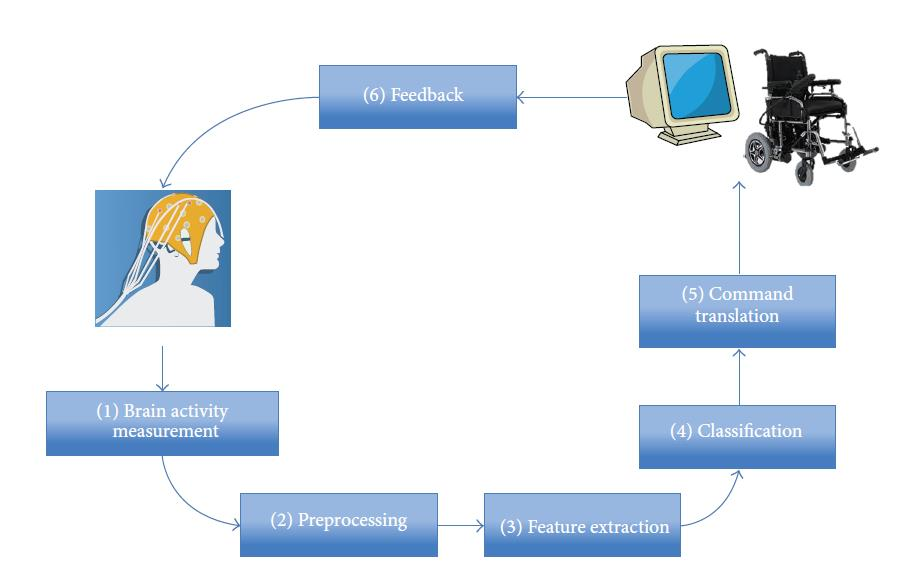
\includegraphics[width=\linewidth]{Figures/BCI_Flow.jpg} % Figure image
%	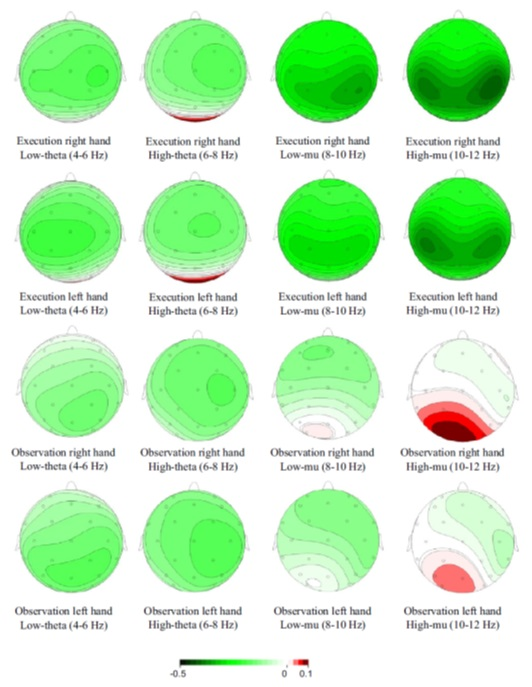
\includegraphics[width=14cm]{Figures/ScalpSignals.jpg} % Figure image
	\caption{Flow diagram of the operation of a typical BCI. (Figure taken from \citep{Martisius2016}.) }
	\label{BCI_F} % Label for referencing with \ref{bear}
\end{figure}

Currently, there are two main methods used in BCI for the feature extraction and classification. These are the Evoked Potentials (EP) and the Oscillatory or Motor Imagery EEG. 

\subsubsection{\bf{Evoked Potentials (EP):}}
Evoked Potential (EP) refers to techniques used to determine the brain activity after an external stimulus. There are two broad techniques of EP used in BCI. These are the Event Related Potentials (ERP) and the Visually Evoked Potentials (VEP).

\vspace {15pt}
\textbf{Event Related Potentials (ERP):}

In an ERP system, the brain response is examined after an external stimulus event. This response is a direct result of the stimulus. ERPs are very small compared to the background EEG activity, therefore, it is needed to average multiple ERPs to extract a clean ERP waveform \citep{Sanei2007}. ERP waveforms are characterized by a number of positive (P) peaks and negative (N) peaks and a number identifying the typical latency of the peak in ms or 100ms. A common ERP BCI system is the P300, which is based on the positive P3 part of the ERP waveform. The P300 BCI system is very common in EEG games \citep{Kerous2018}. A typical ERP waveform is shown in Figure \ref{ERP_F}. The negative voltages in ERP waveforms are usually shown on the upper part of the waveform.

\begin{figure}
	\centering
%	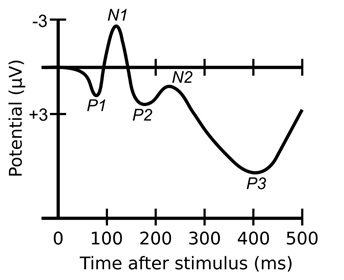
\includegraphics[width=\linewidth]{Figures/ERP.jpg} % Figure image
	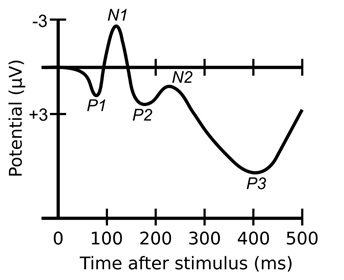
\includegraphics[width=10cm]{Figures/ERP.jpg} % Figure image
	\caption{A typical ERP waveform. (Figure taken from  \citep{Sanei2007}.) }
	\label{ERP_F} % Label for referencing with \ref{bear}
\end{figure}

EEG signals due to background brain activities, as well as artefacts and external signals are considered as noise with white noise characteristics. ERP signals are very weak compared to the rest of the recorded EEG signals, resulting in a low SNR. Therefore, to be able to interpret the ERP signal correctly it is necessary to increase the SNR. This is achieved by repeated trials and averaging the ERP signal. This is true given that the latency and shape of the ERP waveform does not change between trials and that the noise behaves as a zero-mean Gaussian noise.


\vspace {15pt}
\textbf{Visually Evoked Potentials (VEP):}

Visually Evoked Potentials (VEP) share the same characteristics with ERP, in the sense that both require averaging the EEG signals that are time-locked to a stimulus. The stimulus in this case is a light or a visual source. VEP is mainly used in ophthalmology.  

\subsubsection{\bf{Oscillatory or Motor Imagery (MI) EEG:}}
Motor Imagery (MI) BCI refers to BCI systems where motor imagery task being carried out are expressed as changes in the mu (alpha) and the beta frequency bands. When a mental activity results in an increase in a frequency band, this is called event-related synchronization (ERS). On the other hand, if the mental activity results in a decrease in a frequency band, then this is called event-related desynchronization (ERD).  MI BCI are widely used in medical applications, as well as in EEG games. 
Medical applications of MI BCI cover a wide range. Typical applications are, for example, the assistance in the rehabilitation of stroke patients using MI assisted with robotic feedback  \citep{Kai2010}. Another application is the use of MI BCI to control the operation of a wheelchair  \citep{Gala2008}.
The main function in an MI BCI is the classification of the imagery task, that is, the method that will enable the BCI identify the motor imagery task. A variety of methods are being used in order to determine the imagery task ranging from the analysis of the ERS/ERD activity in relation to the frequency band and the electrode positions used to record the EEG signal  \citep{Wolpaw2004, Pfurtscheller2006}, to artificial intelligence techniques, such as machine learning and fuzzy systems  \citep{Xu2009}. Furthermore, since classification requires the analysis of EEG signals recorded from different scalp areas with their spectrum changing with time, digital signal processing tools, such as the wavelet transforms  \citep{Ahmadi2012} are being used.  

\subsubsection{\bf{EEG based Games:}}
In recent years, the developments in smart and mobile devices, as well the success of BCI research in detecting correctly brain activity, resulted in the creation of a new sector in computer game technology. As noted in a review paper \citep{Ahn2014}, BCI games is a rapidly growing field used by healthy people, while there is a tremendous increase in the production of BCI related research papers, due to the availability of a variety of BCI game low price equipment. Some of the main manufactures of BCI game equipment are “Neurosky Mindset” (www.neurosky.com) and “Emotiv EPOC” (www.emotiv.com).  The complexity of the available BCI game equipment ranges from simple 1-electrode/sensor headsets to more complex devices with more than 16 electrodes/sensors. The control paradigms employed in implemented BCI games are the ERP/P300, the Motor Imagery and the Steady State Visual Evoked Potential (SSVEP).




%\begin{table}
%\caption{The effects of treatments X and Y on the four groups studied.}
%\label{tab:treatments}
%\centering
%\begin{tabular}{l l l}
%\toprule
%\tabhead{Groups} & \tabhead{Treatment X} & \tabhead{Treatment Y} \\
%\midrule
%1 & 0.2 & 0.8\\
%2 & 0.17 & 0.7\\
%3 & 0.24 & 0.75\\
%4 & 0.68 & 0.3\\
%\bottomrule\\
%\end{tabular}
%\end{table}


















%DDM model as well as detailed description
%of the DDM-CMP implementation and estimated performance results. The experimental 
%results show that, for the workload tested, the DDM-CMP architecture is able to achieve
%higher speedup values at lower power consumption levels comparing to traditional
%architectures. 

%While our previous work focused on the DDM model [2,3,12] and more recently on high-level %issues of DDM-CMP [5,6], such as estimations of the performance and power benefits, in this %paper we go a step further and present an analysis of the hardware budget for the DDM-CMP. As %a result we can now accurately determine the number of cores that may be included in a chip %with the same hardware budget as other traditional CPUs. In this paper we show that, in the %same hardware budget of a modern high-end single-chip microprocessor, it is possible to build %a DDM-CMP chip with 16 cores. The extra hardware cost for supporting execution under the DDM %model are shown to be less than 17\% of the total area. Moreover, we present and validate the %Runtime Support System of DDM-CMP. A careful design of this system allows the execution of %both regular and DDM applications without any modification to the CPU or the OS. This system %was validated using a functional Simics-based~\cite{simics} full system simulator.

%The rest of this paper is organized as follows. Section~\ref{sec:dataflow} presents 

